\documentclass[fleqn]{article}
\usepackage[nodisplayskipstretch]{setspace}
\usepackage{amsmath, nccmath, bm}
\usepackage{amssymb}
\usepackage{enumitem}
\usepackage{etoolbox}
\usepackage[normalem]{ulem}
\usepackage[hidelinks,colorlinks=true,urlcolor=blue,linkcolor=black]{hyperref}
\usepackage{graphicx}
\usepackage{float}
\usepackage{changepage}
\usepackage{environ,capt-of}

\let\oldfigure\figure% Store original figure float environment
\let\endoldfigure\endfigure
\RenewEnviron{figure}[1][H]{% Update figure environment
  %\par\vspace{\intextsep}% Assume in-text placement, so insert appropriate vertical spacing
  \noindent
  % \patchcmd{<cmd>}{<search>}{<replace>}{<success>}{<failure>}
  \patchcmd{\BODY}{\caption}{\captionof{figure}}{}{}% Replace \caption with \captionof{figure} inside \BODY
  % Set "figure"
  \begin{minipage}{\linewidth}
    \BODY
  \end{minipage}
  %\par\vspace{\intextsep}% Assume in-text placement, so insert appropriate vertical spacing
}

\makeatletter
\begingroup
  \catcode`\$=6 %
  \catcode`\#=12 %
  \gdef\href@split$1#$2#$3\\$4{%
    \hyper@@link{$1}{$2}{\uline{$4}}% or \underline
    \endgroup
  }%
\endgroup

\newcommand{\zerodisplayskip}{
	\setlength{\abovedisplayskip}{0pt}%
	\setlength{\belowdisplayskip}{0pt}%
	\setlength{\abovedisplayshortskip}{0pt}%
	\setlength{\belowdisplayshortskip}{0pt}%
	\setlength{\mathindent}{0pt}}
	
\title{Homework 4}
\author{Owen Sowatzke}
\date{March 29, 2024}

\begin{document}

	\offinterlineskip
	\setlength{\lineskip}{12pt}
	\zerodisplayskip
	\maketitle
	
	\begin{enumerate}
		\item Show that if the activation function of the hidden layer is linear, a three layer network is equivalent to a two layer one.
		
		\begin{figure}[H]
			\centerline{\fbox{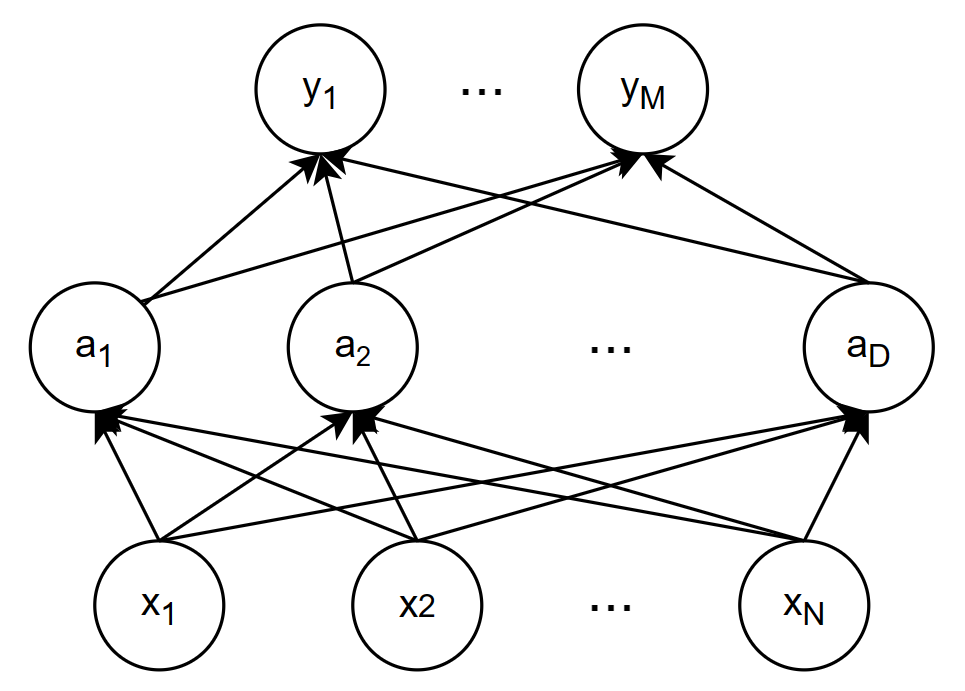
\includegraphics[width=0.4\textwidth]{neural_network_3_layer.png}}}
			\caption{3-Layer Neural Network}
			\label{neural_network_3_layer}
		\end{figure}
	
		The output of the neural network is given by $\mathbf{y} = Q_1(\mathbf{F_1}Q_2(\mathbf{F_2}\mathbf{x}))$ where $Q_2(\boldsymbol{\alpha})$ is the activation function of the hidden layer.
		
		If $Q_2(\boldsymbol{\alpha})$ is linear it can be rewritten as $\mathbf{H}\boldsymbol{\alpha}$. If we substitute this expression for the hidden layer into the above formula, we get the following:
		
		$\mathbf{y} = Q_1(\mathbf{F_1}Q_2(\mathbf{F_2}\mathbf{x})) = Q_1(\mathbf{F_1H(F_2\mathbf{x})}) = Q_1(\mathbf{F_1HF_2x}) = Q_1(\mathbf{Ax})$
		
		where $\mathbf{A} = \mathbf{F_1HF_2}$.
		
		Therefore, the neural network is equivalent to two-layer neural network.
		
		\begin{figure}[H]
			\centerline{\fbox{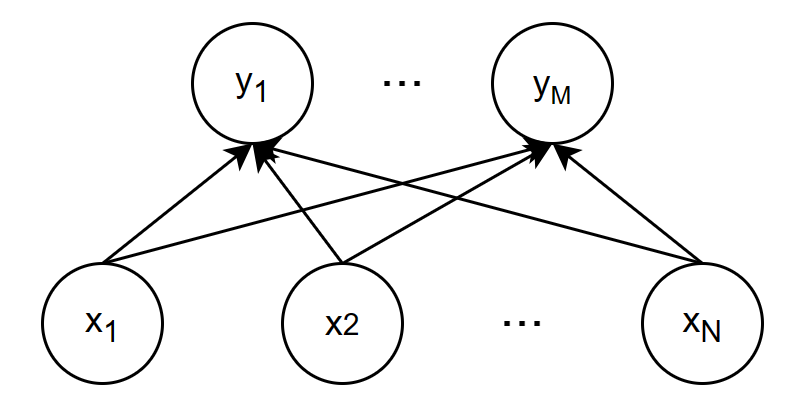
\includegraphics[width=0.4\textwidth]{neural_network_2_layer.png}}}
			\caption{2-Layer Neural Network}
			\label{neural_network_2_layer}
		\end{figure}
		
		\item Assume that a network produces the output $y_i$ in response to the i-th training image from class 1, and the output $x_i$ in response to the i-th training image from class 2. We wish to train the network to maximize the cost function $J(\text{net}) = \frac{\sum_{i=1}^{N}{y_i^2}}{\sum_{i=1}^{N}{x_i^2}}$. Derive the gradient for this cost function and describe how the network updates might be made using batch training and a single image at a time.
		
		We can re-express the gradient in matrix-vector notation as follows:
		
		\begin{equation*}
			J(\text{net}) = \frac{\mathbf{y}^T\mathbf{y}}{\mathbf{x}^T\mathbf{x}}
		\end{equation*}
		
		where $\mathbf{x} = \begin{bmatrix}x_1 & x_2 & \cdots & x_N \end{bmatrix}^T$ and $\mathbf{y} = \begin{bmatrix}y_1 & y_2 & \cdots & y_N \end{bmatrix}^T$
		
		\begin{equation*}
			\nabla_{\mathbf{y}}{J} = \frac{2\mathbf{y}}{\mathbf{x}^T\mathbf{x}} \ \text{and}\ \nabla_{\mathbf{x}}{J} = -\frac{2\mathbf{x}\mathbf{y}^T\mathbf{y}}{(\mathbf{x}^T\mathbf{x})^2}
		\end{equation*}
		
		Define $\mathbf{z} = \begin{bmatrix} \mathbf{y} \\ \mathbf{x} \end{bmatrix}$. Then, we can express $\nabla_{\mathbf{z}}{J}$ as follows:
		
		\begin{equation*}
			\nabla_{\mathbf{z}}{J} = \begin{bmatrix}
				\frac{2\mathbf{y}}{\mathbf{x}^T\mathbf{x}} \\[3pt]
				-\frac{2\mathbf{x}\mathbf{y}^T\mathbf{y}}{(\mathbf{x}^T\mathbf{x})^2}
			\end{bmatrix}
		\end{equation*}
		
		In other words
		
		\begin{equation*}
			\frac{\partial{J}}{\partial{y_i}} = \frac{2y_i}{\sum_{i=1}^{N}x_i^2}\ \text{and}\ \frac{\partial{J}}{\partial{x_i}} = -\frac{2x_i\sum_{i=1}^{N}y_i^2}{\left(\sum_{i=1}^{N}x_i^2\right)^2}
		\end{equation*}
		
		The network updates can be made using batch training or a single image at time. When using batch training, the gradient is averaged over all the training images before an update is made. Conversely, when using a single image at a time, the updates are made after each training image is processed using the gradient for that image. In either case, the gradient (or average gradient) can be computed with respect to each of the neural network's intermediate parameters using backpropogation. (Backpropogation computes the intermediate gradients by applying the chain rule). Once each of the gradients have been computed, gradient descent can be used to update each of the weights.
		
		\item Using the IRIS data set available at \href{https://en.wikipedia.org/wiki/IRIS_flower_data_set}{https://en.wikipedia.org/wiki/\\IRIS\_flower\_data\_set}, design a neural network classifier. The network should have two fully connected layers. The first layer should have 2 input neurons and 5 output neurons. The second layer should have 5 input neurons and 3 outputs neurons. For each input, the output should be a 3 element vector with "1" for the correct class, and "0" corresponding to the other two classes. You may use 40 samples from each class for training, and test with the remaining. Use the ReLu function as the nonlinearity between the layers.
		
		For the computer exercise, the neural network required only 2 of the 4 features. Therefore, I had to chose 2 features from the input dataset. I chose features 3 and 4 because they resulted in better classification accuracy.
		
		\pagebreak
		\begin{enumerate}
			\item[1)] Tabulate the results in terms of classification accuracy
			
			\begin{figure}[H]
				\centerline{\fbox{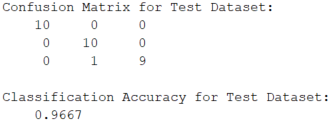
\includegraphics[width=0.8\textwidth]{test_data_results.png}}}
				\caption{Test Data Results Output by Function}
				\label{test_data_results}
			\end{figure}
		
			Referring to the figure above, the classification accuracy for the test data was 96.67\%.
			
			\item[2)] What are the number of parameters that the network must learn? How does that compare to the amount of training data?
			
			The network must learn a $2 \times 5$ matrix plus a $5 \times 1$ bias for the first fully connected layer and a $5 \times 3$ matrix plus a $3 \times 1$ bias for the second fully connected layer. Thus, the network must learn a total of 33 parameters. This is as significant number of parameters given the size of the training data set (120). Specifically, the number of learnable parameters is 27.5\% the size of the training data set. 
			
			\item[3)] How accurate is the training process, and how does it compare to the test results?
			
			\begin{figure}[H]
				\centerline{\fbox{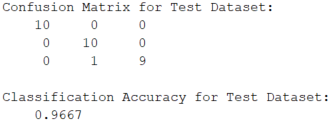
\includegraphics[width=0.8\textwidth]{test_data_results.png}}}
				\caption{Training Data Results Output by Function}
				\label{training_data_results}
			\end{figure}
		
			Referring to the figure above, the classification accuracy for the training data was 95.83\%. This is roughly the same as the test data set, which implies that the training data set is representative of the test data set. The slight performance decrease for the training data set is most likely due to the random selection of training data.
			
		\end{enumerate}
		
		Submit your code along with your answers.
	\end{enumerate}
\end{document}